% !TeX encoding = UTF-8
% !TeX program = pdflatex
% !TeX spellcheck = en_US

\documentclass[LaM,binding=0.6cm]{sapthesis}
\usepackage{float}
\usepackage{microtype}

\usepackage{hyperref}
\hypersetup{pdftitle={Arrhythmia classification from ECG signals},pdfauthor={Angelo Catalani}}

% Remove in a normal thesis
\usepackage{lipsum}
\usepackage{curve2e}
\definecolor{gray}{gray}{0.4}
\newcommand{\bs}{\textbackslash}

% Commands for the titlepage
\title{Arrhythmia classification from ECG signals}
\author{Angelo Catalani}
\IDnumber{1582230}
\course{Engineering in Computer Science}
\courseorganizer{Dipartimento di Informatica, Automazione e Gestionale}
\AcademicYear{2018/2019}
\copyyear{2013}
\advisor{Prof. Aris Anagnostopoulos}
\coadvisor{Prof. Ioannis Chatzigiannakis}
\authoremail{catalaniangelo@gmail.com}

\examdate{15 July 2019}
\examiner{Prof. Nome Cognome}
\examiner{Prof. Nome Cognome}
\examiner{Dr. Nome Cognome}
\versiondate{\today}



\begin{document}

\frontmatter

\maketitle

\dedication{Dedicated to\\ my parents}

\begin{abstract}
A programmer is a problem solver and its activity requires a high level of creativity as well as multidisciplinary knowledge.\\This project gave me the opportunity to implement innovative algorithms for medical purposes: I strongly believe in technological advancement as the key to improve the quality of life and world around us.
\end{abstract}

\begin{acknowledgments}
I would like to express my special thanks of gratitude to my professors (Aris Anagnostopoulos and Ioannis Chatzigiannakis) who gave me the golden opportunity to do this wonderful project.\\Secondly, I would also like to thank my parents and relatives who sustained me a lot over my studies.
\end{acknowledgments}

\tableofcontents



\mainmatter

\chapter{Introduction}
Cardiovascular diseases (CVDs) are the first cause of death worldwide: 18 million people died from CVDs in 2016, representing 31\% of all global deaths (\cite{who}).\\This project is focused on the cardiovascular diseases related to complications with the electrical system that regulates the steady heartbeat and generates abnormal heartbeats called arrhythmias.\\A great deal of people, during life, can experience irregular heartbeats and generally,  they are harmless and happen in healthy people free of heart disease.\\However, some abnormal heart rhythms can be serious or even deadly.\\A standard tool to diagnose arrhythmias is the electrocardiogram (ECG): measurement of the heart's electrical activity.\\Since it is a non-invasive and painless test for the patients, it can be employed to collect massive volumes of data, and subsequently analyze them, with the purpose of automatically detecting arrhythmias.\\The equipment to produce electrocardiograms is principally present in hospitals, where cardiologists use their knowledge and experience to carefully evaluate the ECG. However, this activity is time-consuming and prone to error: an automatic approach can support them during their decision.\\In addition to this, accurate and low-cost diagnosis of arrhythmic heartbeats is highly desirable since it can detect early heart problems and prevent dangerous consequences. This is the reason it is not surprising recent literature is focused on this topic.\\In general, the ECG's analysis is constituted of two phases:
\begin{enumerate}
\item beat detection: extrapolate the temporal segment of the ECG related to the contraction of the heart
\item arrhythmia  classification: detection of arrhythmic beats
\end{enumerate} 
This work is concentrated only on the latter, that is more challenging because until now, there is not any perfect solution to the problem.\\We propose a series of algorithms able to automatically detect arrhythmias, with the aim for the future, to implement them on wearable devices.
In paritcular
\section{Document Structure}
In \textbf{Chapter 2}, I will discuss the heart's anatomy and the shape of beats and arrhythmias in a ECG.\\Then in \textbf{Chapter 3} and \textbf{Chapter 4}, I will cover pre-processing and feature extraction techniques applied to the ECG, to improve:
\begin{enumerate}
\item information's quality: signal filters and discrete wavelet transform
\item classification performance: data augmentation 
\end{enumerate}
In \textbf{Chapter 5} I will describe the implemented algorithms, with the corresponding results, mainly based on Random Forest, Support Vector Machine and Neural Network.\\Finally, in \textbf{Chapter 6}, I will compare some of the best models found in the literature with my approaches: the latter take advantage of the last advancement in Machine Learning and reach the state of art's performance.


\chapter{Principles of ECG Evaluation}
This chapter explains the underlying mechanism behind the heart beating and how this process is visible on the ECG. The importance of this argument, relies on the consequent ability to define the ECG's key features for arrhythmias detection.

\section{Heart's Anatomy }

The human heart pumps blood to the body, as the result of electrical impulse and mechanical response, due to conductive and mechanical cells. The contraction is possible only in presence of an electrical stimulus but in some pathological case the inverse is said to be true. This is the reason why to determine the health state of this muscle, it is of paramount importance to asses both the mechanical and electrical functions.The first one can be monitored with blood pressure, pulses while the latter with the ECG.\\The ECG's relevance, is the possibility to have a graphic display of the electrical activity in the heart, so that it is possible to identify arrhythmias as recognizable patterns. For example, it is straightforward to presume the ECG of Fig. ~\ref{fig:ecgex} contains 5 beats.
\begin{figure}[H]
	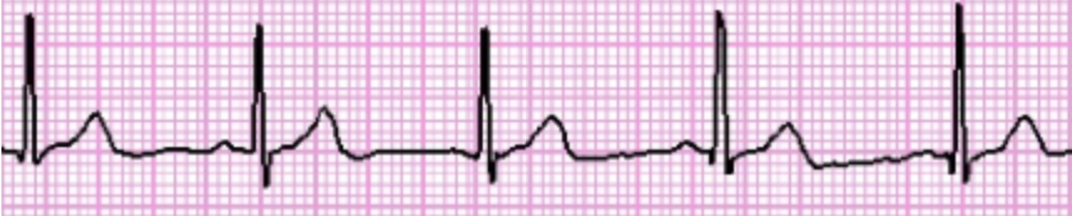
\includegraphics[width=50mm,scale=0.7]{ecgtrace}
	\caption{Example of ECG trace}
	\label{fig:ecgex}
\end{figure}

\subsection{Electrical Cell}
This cells have the exclusive capability to discharge electrical current without the necessity of external stimuli: this property is called automaticity , and the underlying mechanism is the sodium pump.\\In a resting cardiac cell the electrical charges are equally balanced and there is not electrical flow: the cell is said to be polarized or in the ready state.\\The automaticity property, allows this cell to modify the membrane and pull sodium inside and potassium outside, so that the resulting difference of potential causes an electrical flow: this is the basic sodium pump functionality that makes the cell in a state called depolarized or discharge state.\\Finally, after this step, the process to turn the depolarized state in the original restring one, is called repolarization and it consists of pulling out of the cell's membrane the  sodium and inside the potassium, bringing in the end the cell to the original resting state. The whole process is described in Fig. ~\ref{fig:ecgtrans}.  
\begin{figure}[H]
	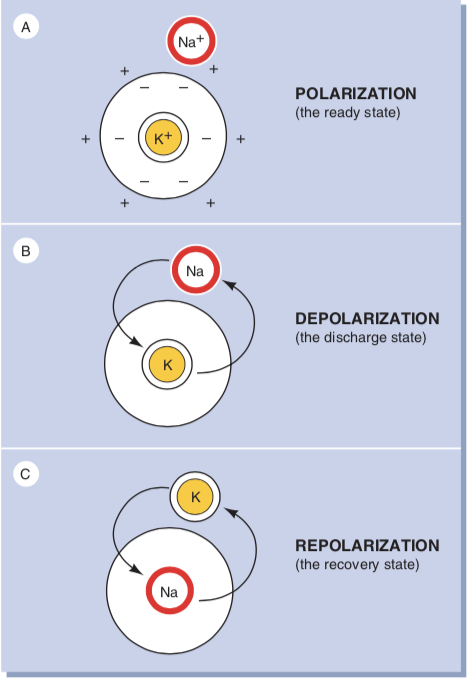
\includegraphics[width=50mm,scale=0.7]{ecgtrans}
	\caption{Electrical cell transactions: \cite{ecgbook}}
	\label{fig:ecgtrans}
\end{figure}
The heart is made of 4 chambers: two atriums in the upper part and two ventricles downside.The electrical cells conduct the current flow through a set of connections that overall constitute the conductive system and completely cover the heart's surface: this allows the consequent contraction of atriums and ventricles.
\subsection{Heartbeat Cycle}
Normally, the electrical impulse is produced in the sino atrial (SA) node positioned in the upper part of the right atrium. Then, it propagates down to the right atrium with the inter nodal pathways to reach the atrio ventricular node (AV) and left with  the inter atrial pathways to reach the left atrium. The entrance to the left and right ventricles is provided by the Bundle of His, through the left and right bundle branch, that terminates with Purkinje fibers who are in charge to contract the ventricles.\\It is interesting to note not all the portion of the heart have the same beat rhythm (beats per minute):
\begin{enumerate}
\item SA node: 60-100  
\item AV node: 40-60 
\item Ventricles: 20-40 
\end{enumerate}
The discussed structure is depicted in in Fig. ~\ref{fig:hearts}.
\begin{figure}
	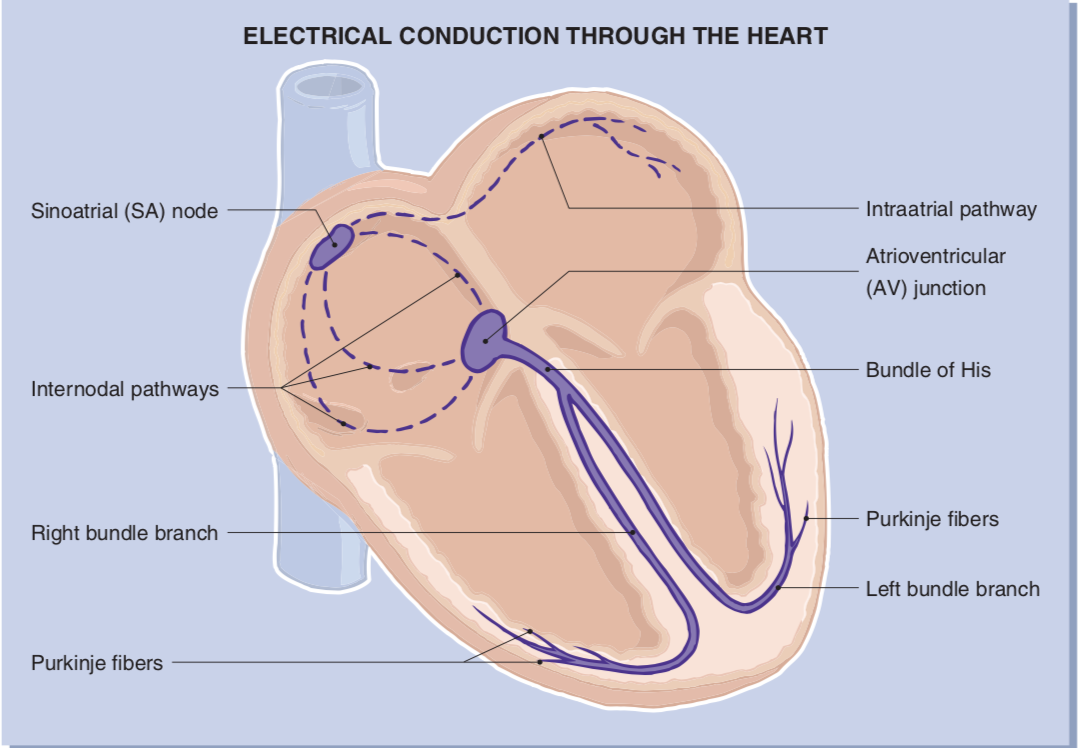
\includegraphics[width=50mm,scale=0.7]{heartex}
	\caption{Electrical tissue of heart: \cite{ecgbook}}
	\label{fig:hearts}
\end{figure}
In the ECG, in normal condition, the visible beat rate is due to SA node because it has the highest frequency and overrides all the other: this is the reason why it is defined as the pacemaker.
The above values are called inherent rates and can help us to infer heart's dysfunctions visible in the ECG as a different SA rhythm. In a pathological context, for example if the SA node fails, the pacemaker becomes the AV node and  a slower rhythm is visibile on the ECG: this callback safety mechanism is named escape.

\section{ECG tracing}
The acquired knowledge in the previous subsection, is essential to investigate how the electrical activity is transferred to graph paper to be analyzed for our task.\\The ECG is obtained placing some electrodes on the patient skin and connecting it, to a machine that will display the electrical activity.\\The location of the electrodes is crucial for the final output and it is possibile to obtain multiple views ( or lead) of the same heart, just by varying their position.\\In particular, some arrhythmias are more visible on a given view, and in general an effective diagnosis interpolate more leads. For example, in the dataset we consider, each ECG has two leads:
\begin{enumerate}
\item modified limb lead II (MLII) where the electrodes are on the chest.
\item modified chest lead V1 (MCL1) where negative electrode is placed close to the left shoulder and the positive electrode to the right of the sternum 
\end{enumerate}
For a long time, the most adopted lead has been the Lead II, and in the following I will take into consideration this configuration. However, there are different leads with better effectiveness.\\In Lead II the negative electrode is placed to the right, above the heart, while the positive to the left, behind the heart. In this way, when the electrical impulse propagates from the atrium to the ventricle, the ECG device will display an upright wave, while an upside down shape is generated in the opposite case (Fig. ~\ref{fig:ruleflow}).
\begin{figure}[H]
	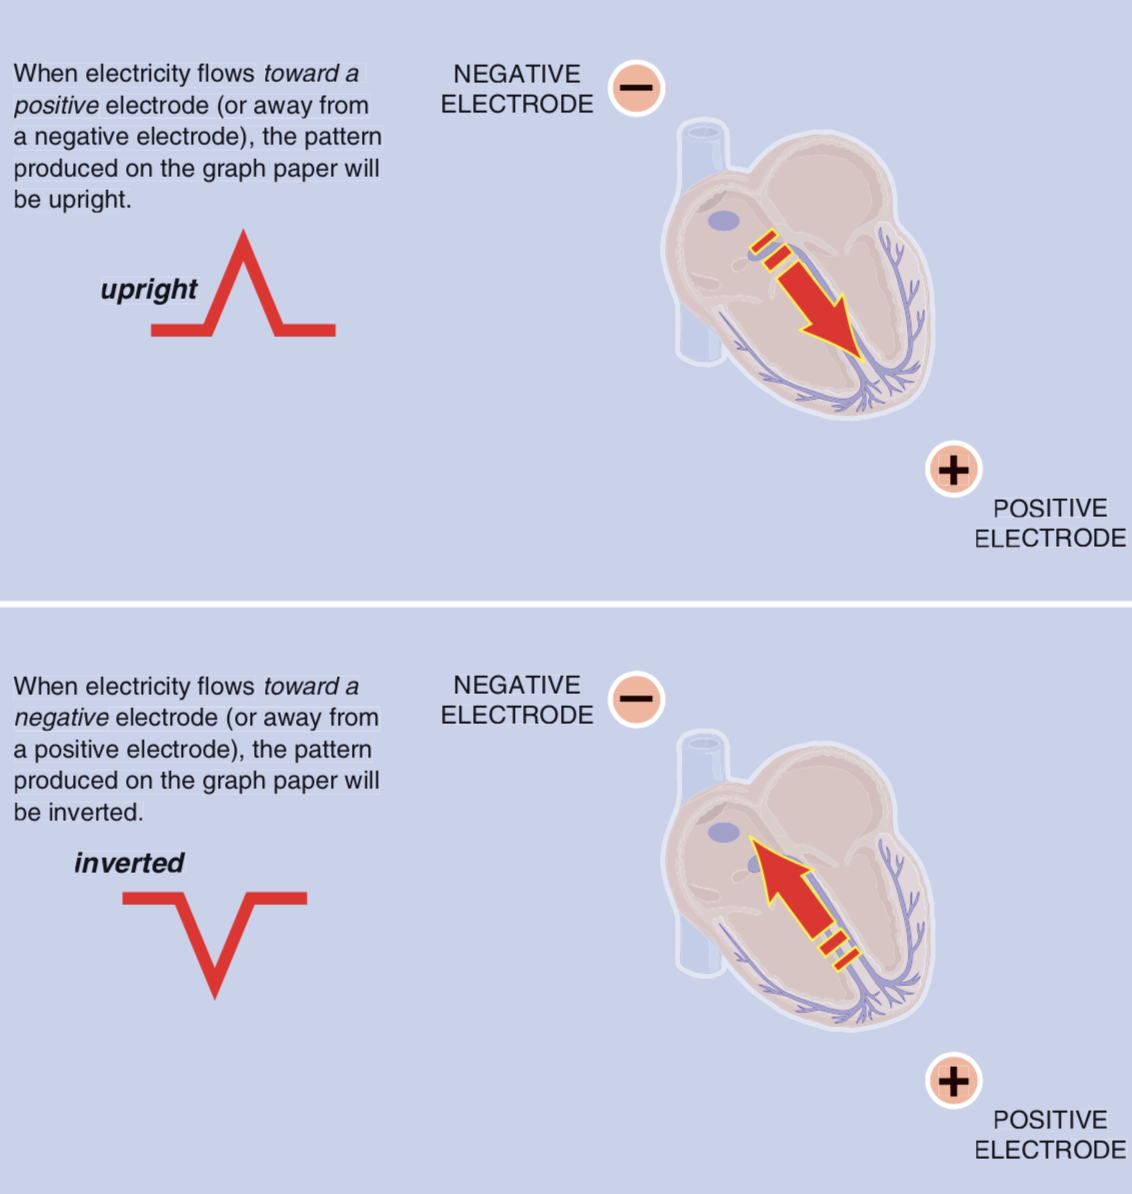
\includegraphics[width=50mm,scale=0.7]{ruleflow}
	\caption{Lead II basic principles: \cite{ecgbook}}
	\label{fig:ruleflow}
\end{figure}
Finally, the ECG is written on a conventional graph paper (Fig. ~\ref{fig:ecgtrace}) where the voltage levels are measured comparing the horizontal lines, and the time interval, considering the vertical lines: two consecutive vertical splits cover 0.04 seconds.
\subsection{Heartbeat Shape}
During a normal beat, the heart first enter in the atria and then into the ventricles: this requires a synchronized mechanism so that while the atria fill, the ventricles contract and viceversa. During each phase of the cardiac cycle, a distinct pattern is produced on the ECG graph paper. This pattern describes instantly what is happening in the heart and it has the shape depicted in Fig. ~\ref{fig:beatshape}.
\begin{figure}[H]
	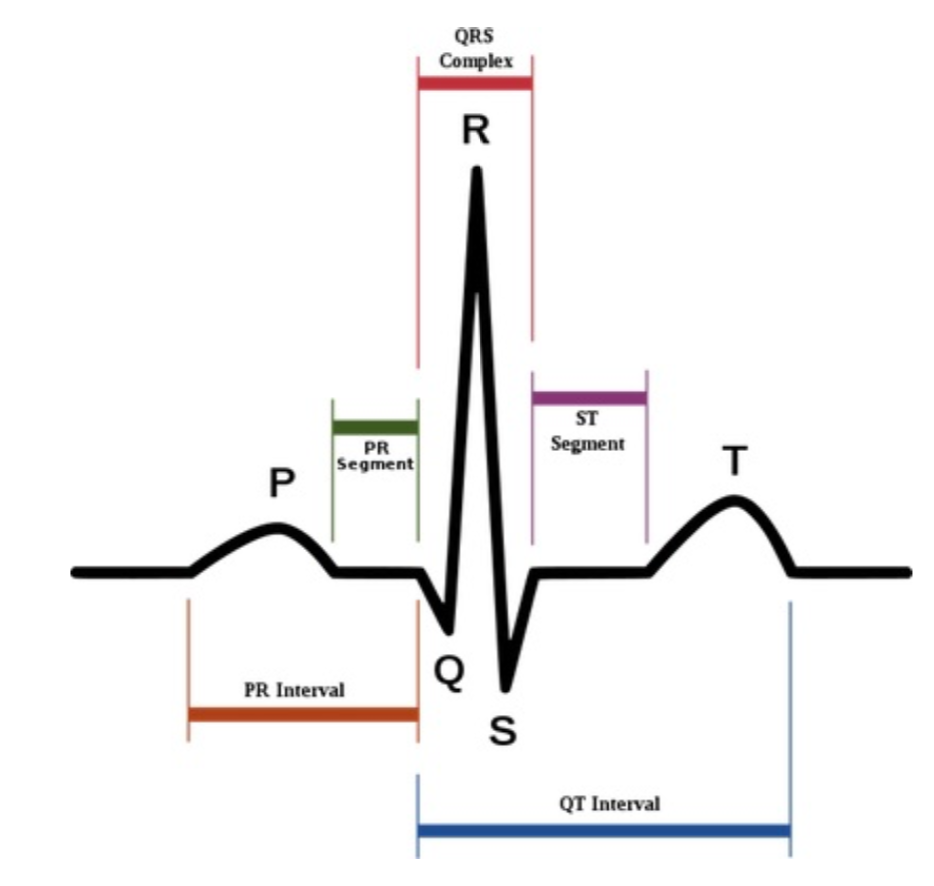
\includegraphics[width=50mm,scale=0.7]{beatshape}
	\caption{Heartbeat in the ECG}
	\label{fig:beatshape}
\end{figure}
The beat shape starts with a deflection: the P wave and it is generated by the SA node. Subsequently the impulse leaves the atria to reach the AV node and it encounters a slight delay because the encountered electrical tissues are slower. This is translated into a short period of electrical inactivity called the PR segment.\\The subsequent wave is the QRS complex, due to ventricular depolarization and it is significantly larger than the P wave because to  ventricles are greater than atria, so that more potential energy is required. The Q wave is defined as the first negative deflection following the P wave but before the R wave. The Q wave flows immediately into the R wave, which is the first positive deflection following the P wave. Next comes the S wave, which is defined as the second negative deflection following the P wave, or the first negative deflection following the R wave.\\After the ventricles depolarize, they begin their repolarization phase, which results in another wave in the ECG. The T wave is indicative of ventricular repolarization.\\The atria also repolarizes, but this event is not significant enough to show up in the ECG.\\Between the S and the T wave is a section called the ST segment. The ST segment is the flat, isoelectric section of the ECG between the end of the S wave and the beginning of the T wave. It represents the interval between ventricular depolarization and repolarization, and anomalies in this segment are symptom of infarction.

\subsection{Type of Arrhythmias}
Arrhythmia analysis is a complex task due to the high variability of the heart's mechanism inside each patient. Arrhythmias are classified into two classes:
\begin{enumerate}
\item rhythmic: constituted of a series of irregular beats
\item morphological: single abnormal beat
\end{enumerate}
This work is concentrated on the latter.\\Morphological arrhythmias are classified into 4 macro classes by the Association for the Advancement of Medical Instrumentation (AAMI) standard, with respect to the location where the anomaly starts:
\begin{enumerate}
\item N-class. It happens when the beat regularly starts at the SA node but can be blocked in the left or right bundle branch.It includes regular beat.For example, left bundle brach block, happens when the impulse does not reach the left ventricle because the left bundle is compromised: in this situation , first the right ventricle will depolarize and then also the left one. This results in a QRS complex longer than 120 ms.
\item S-class. It happens when the impulse starts below the SA node: in this situation the impulse will begin at the bottom and subsequently will reach the upper part, resulting in an upside down P wave.
\item V-class. It happens when the impulse originates in the ventricles and it shows up in the ECG as a tall and wide QRS
\item F-class. It happens when there are multiple sources of depolarization: for example in Fig. ~\ref{fig:arrhex} the P wave is modified by an additional source of depolarization
\end{enumerate}
\begin{figure}[H]
	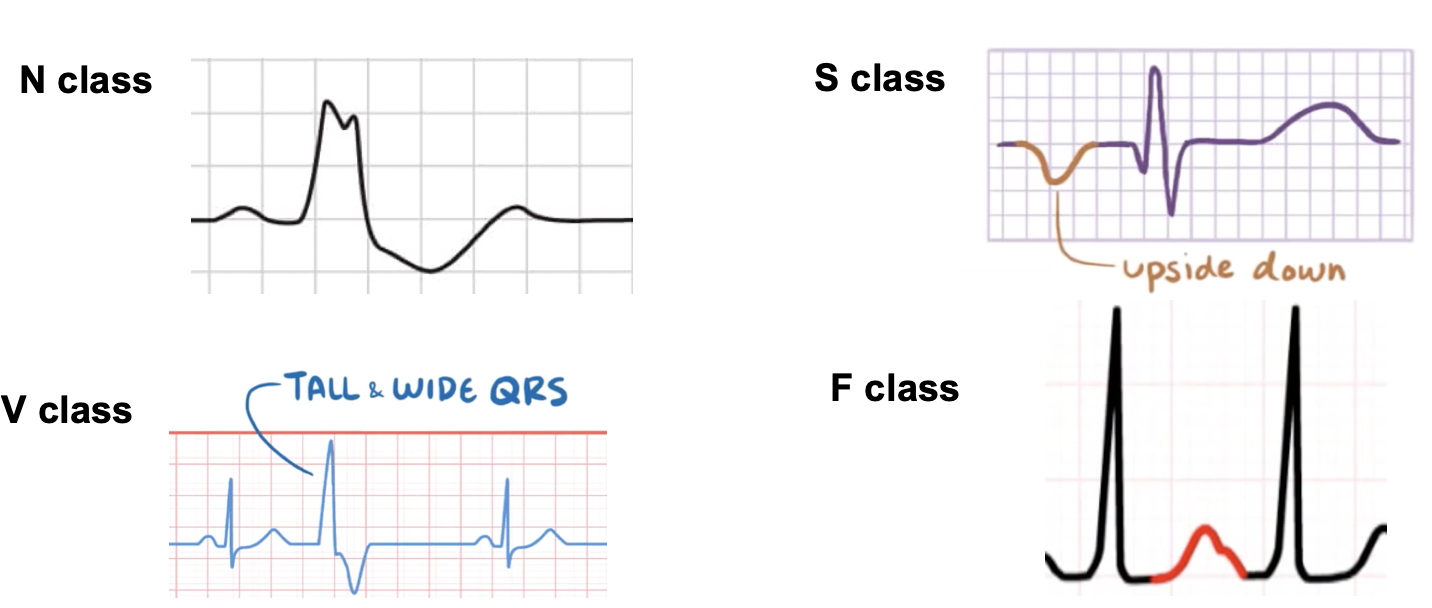
\includegraphics[width=50mm,scale=0.7]{arrhex}
	\caption{Examples of Arrhytmias}
	\label{fig:arrhex}
\end{figure}
A more detailed arrangement of the above classes are depicted in the figure below.
\begin{figure}[H]
	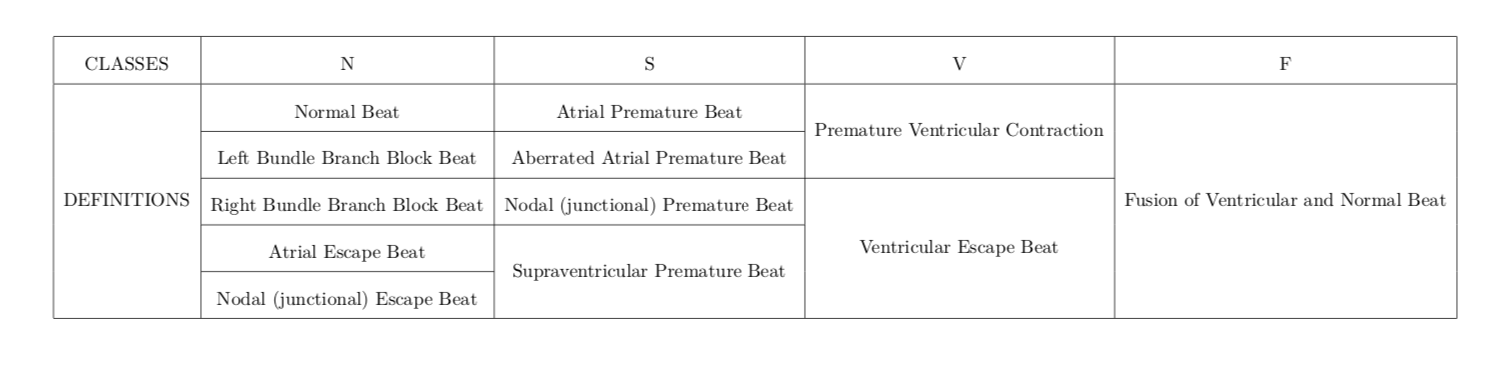
\includegraphics[width=50mm,scale=0.7]{allclass}
	\caption{Detailed classification of arrhythmias }
	\label{fig:allclass}
\end{figure}

\chapter{Pre-Processing}
As we have previously, discussed, the ECG tracing is an empirical process prone to noise measurements whose removal is of high importance to guarantee the detection of the relevant features without incurring into overfitting issues.\\The principal methods to remove noise are based on frequencies domain analysis : in the following I will describe Median Filter and Discrete Wavelet Transform.\\In addition to this, the dataset we are taking into consideration is highly over balanced: one class constitutes more than 80\% of all the elements: this can lead to inconsistencies because an algorithm could reach high accuracy, merely predicting only that class without any generalization competence.\\For the purpose of handling the latter, we have used several approaches based on data augmentation and weighted loss function. 
\section{De-Noise}
The ECG  can be affected by several sources of noise during the recording, attributable to : 
\begin{enumerate}
\item Baseline wander caused by patient's movements.It is visible in the signal with frequencies below 0.5 Hz (Fig. ~\ref{fig:n1}.a ).
\item Power line interference caused by electromagnetic external devices.It appears in the signal as 50/60 Hz sinusoids (Fig. ~\ref{fig:n1}.b ) .
\item Muscle artifact caused by muscle activity near the electrode for the contraction of the heart's patient. It is difficult to be removed since it is strictly related with the electrical impulse of the ventricles that determines the QRS complex on the ECG. Its removal can result in unwanted distortion of the signal (Fig. ~\ref{fig:n1}.c ) .
\end{enumerate}
\begin{figure}[H]
	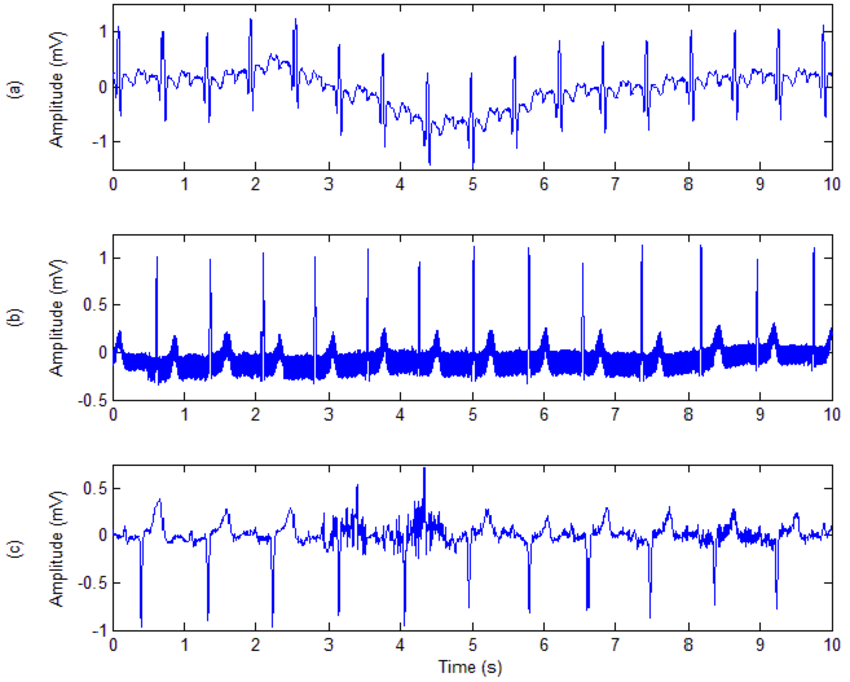
\includegraphics[width=50mm,scale=0.7]{noise.png}
	\caption{Example of noise in ECG recordings. (a) Baseline wander, (b) Power line interference, and (c) Muscle artifact. \cite{noise}}
	\label{fig:n1}
\end{figure}
It is crucial to note the role of de-noise algorithms is to clean the signals without loosing relevant information:  after the processing, the filtered signal must contain the original key features of a beat in terms of P,Q,R,S,T wave.\\In this project we have considered 2 different ways of noise removal : median filter and discrete wavelet transform (DWT).

\subsection{Median Filter}
A median filter takes as input a signal $S = [x_1 , \dots , x_n]$ and a window of size : $w$.\\It returns a converted signal where for every sample : $x_i \in S$, it is computed the median of the elements : $[x_i, x_{i+1}, \dots , x_{(i+w) \; mod \; n}]$.\\The intuition behind a median filter, is that noisy samples tends to have too high or too low values, with respect to the neighbor samples : replacing them with the median in a given range can be a good approach.\\This technique is used in \cite{rfdwt} to mitigate the noise due to baseline wonder.




\subsection{Discrete Wavelet Transform}
The ECG signal is non stationary because beats are generated by the heart under influences of physiological factors that depend on the brain and change continuously over the time.\\In order to characterize the frequency domain of a non stationary signal, the Fourier transform is not perfectly applicable because it is not accurate to assume that a given frequency is equally distributed in the signal: this is only true for periodic, stationary signal.\\In particular, to represent the ECG signal we are interested not only in the frequency contained, but also in the portion of the signal exhibits a given frequency.\\With the aim of having a better resolution in time, it is possible to study the frequencies of the signal present in a temporal window of the signal: for example we can study the frequencies of the signal from $t=0$ to $t=0.1$, so that we can infer the frequencies localized in the interval.\\However, the drawback of this approach is that it is not possible to detect all the frequencies because in that window we can only find the frequencies greater than $\frac{1}{0.1}=10 Hz$ , since for frequencies greater than $10 Hz$ we need to consider a widow larger than: $0.1s$.\\The explained tradeoff between frequency and time resolution is the application of the Heisenberg's Uncertainty Principle.\\In order to mitigate this issues: the optimum approach is to consider small window for high frequencies and large window for low frequencies.\\In fact, when a signal component is rapidly changing it is essential to detect the instant when this happens.\\on the contrary, when a component repeats slowly it is necessarily a larger window to detect it.\\The Discrete Wavelet Transform (DWT) takes advantage of this latter consideration.\\DWT considers as basis function a wavelet instead of sinusoid employed by Fourier Transform.\\A wavelet is a function with with a limited duration : it has an amplitude that begins at zero, increases, and then decreases back to zero. A wavelet is more localized in time than a sinusoid because it exists only in a restricted interval (Fig. ~\ref{fig:we} ). 
\begin{figure}[H]
	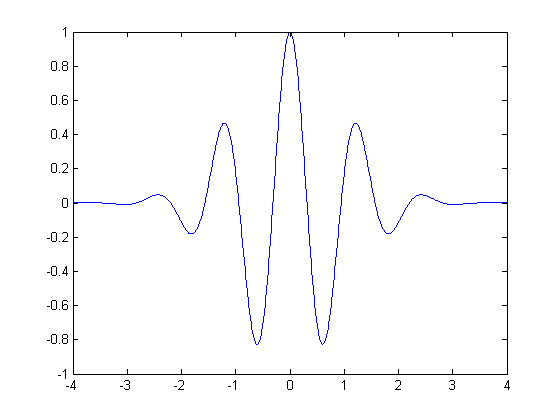
\includegraphics[width=50mm,scale=0.7]{waveletexample.png}
	\caption{Wavelet named Meyer}
	\label{fig:we}
\end{figure}
The main parameters of a wavelet are:
\begin{enumerate}
\item scaling.The scale of a wavelet is a measure of how it is expanded, so that the higher the scale the more it is spread and the less it is localized in time (Fig. ~\ref{fig:ws} ).
\item shifting.The wavelet is shifted across the input signal to align it with the features we are interested in, for example the QRS complex.
\end{enumerate}
\begin{figure}[H]
	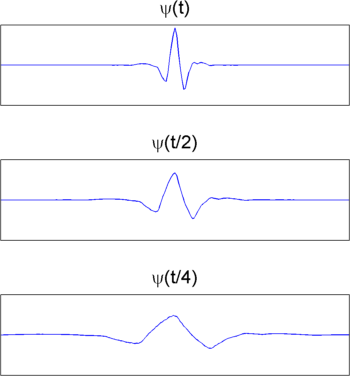
\includegraphics[width=50mm,scale=0.7]{wavescale.png}
	\caption{Wavelet with scaling factor of 1,2,4: \cite{matdwt} }
	\label{fig:ws}
\end{figure}
In general the idea of DWT is to analyze the correlation between the signal and a given wavelet shifted over the signal with increasing scale: initially it is analyzed high frequency behavior and at each successive step the scale is doubled and the signal downsampled for the Nyquist criterion.\\In conclusion, DWT outputs the signal at different bandwidth, such that at each level of analysis, the output is high, if there is a strong correlation of the signal at that frequency with the wavelet at that scale.\\There are several families of wavelet, and the choice of the correct one, relies on the similarity of shape with the portion of ECG we are interested (Fig. ~\ref{fig:wf}) .\\For example, a common choice is the Meyer wavelet (Fig. ~\ref{fig:we} ) because it is comparable to the QRS complex.\\DWT is mainly used as :
\begin{enumerate}
\item a filter ignoring the coefficients at a given frequency level while reconstructing the signal (\cite{lnlf}).
\item feature selection considering the coefficients with high value, or with high correlation with the original signal (\cite{rfdwt},\cite{lnlf}).
\end{enumerate}
\begin{figure}[H]
	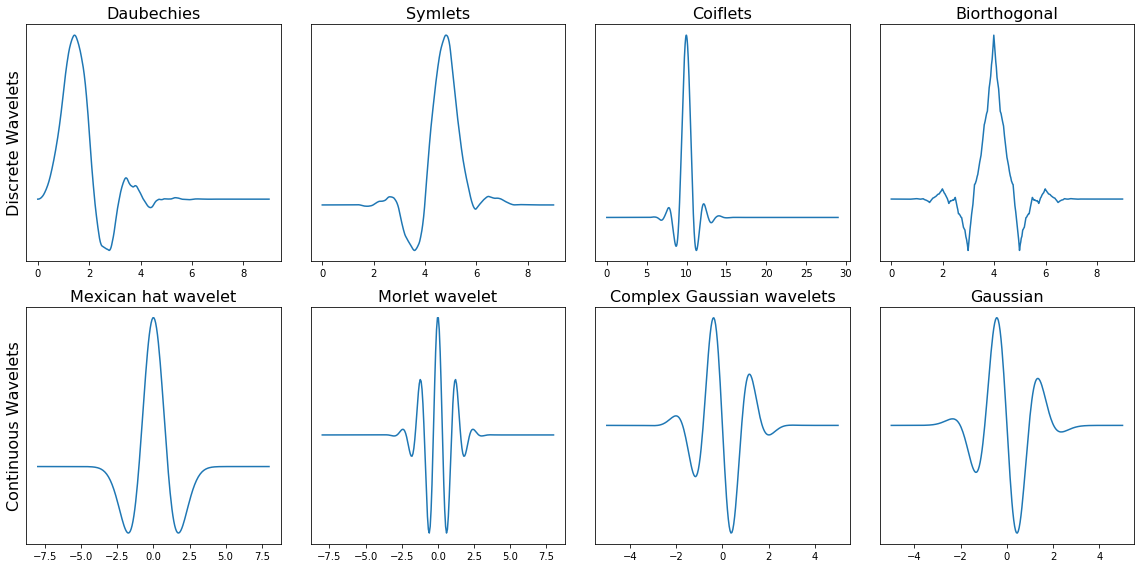
\includegraphics[width=50mm,scale=0.7]{waveletfamilies.png}
	\caption{Wavelet families: \cite{watut} }
	\label{fig:wf}
\end{figure}




\section{Data Augmentation}
The dataset's details will be discussed in chapter \ref{datasec}: so far it is important to note it is overbalanced. In particular the N class is more than 80\% of the whole dataset.\\Models trained on imbalanced dataset do not acquire any generalization power: they are biased toward the most populated class and fail to detect the distinguish features of the others.\\For example in our case, a model could reach a high accuracy during the train just by learning to always predict the same class.\\Class imbalance is typical of biological dataset, where the interest is towards minority samples that are linked to rare events (\cite{onf/ijcnn/HeBGL08}).\\We have tried to solve this issue using the following methods: Smote, Adasyn and weighted loss function for neural networks.\\In the following, I will use the following notation:
\begin{enumerate}
\item Dataset: $D$, with $n$ samples: $D=\{(x_1,y_1),\dots,(x_n,y_n)\}$
\item Classes: $Y=\{1,-1\}$ such that $|y_i \in Y$. For now we consider only two classes, but the same considerations can be generalize to $N$ classes 
\item $m_s$ and $m_l$ is the number of samples belonging respectively to the under-balanced and over-balanced class: $m_s\leq m_l$ and $m_s+m_l=m$
\end{enumerate}
\subsection{Smote and Adasyn}
In order to build a consistent dataset, it is possible to add new elements to the less populated class (over-sampling), or to remove existing samples of the most populated class (under-sampling). We have adopted the first one, 
to take advantage of all the information contained in the dataset even for unbalanced classes. The main oversampling algorithms are Smote (\cite{smotepaper}) and Adasyn (\cite{conf/ijcnn/HeBGL08}). The latter is an improved version of the first one. \\In general, Smote takes into consideration a given class and generates $N$ additional synthetic examples for each original element. For example, if $N$ is 1, the size of the class is doubled.\\Specifically, this algorithm performs the following steps:
\begin{enumerate}
\item take a sample: $x_i$, and consider the difference vectors $z_1,\dots,z_n$ between $x_i$ and the $K$ closest neighbors of the same class: ${x_j,\dots,x_{j+K}}$. In the end, $z_j = x_i - x_j$  where $1\leq j,i\leq n$
\item for every $N\leq K$, randomly chosen, difference vectors: $z_j$, returns a new sample: $s_j = x_i+r\cdot d_j$ where $r \in [0,1]$ is a random value.
\end{enumerate}
In the end, a new point is a randomly positioned in the segment whose extremities are the original sample and its neighbor.This approach effectively forces the decision region of the minority class to become more general (\cite{smotepaper}). However, Smote does not create representative samples when the under-balanced class has extreme values: in this case the created element will be centered in the dataset space even if the under-balanced samples will probably lie on the boundary.
\begin{figure}[H]
	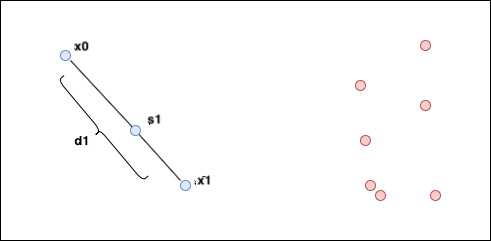
\includegraphics[width=50mm,scale=0.7]{smoteex.png}
	\caption{The blue class is underbalanced: Smote generates a new sample: $s_1$ between $x_0$ and $x_1$}
	\label{fig:smoteex}
\end{figure}
Adasyn is an advanced version of Smote: the main difference is the first automatically detect the number of samples to generate: $g_i$, with respect to the element considered in the under-balanced class: $x_i$.In general, more samples will be created for samples whose neighbors belong to another class. The idea is that missing points should concentrate in the dataset space where a given element is under-represented.\\Specifically, it performs the following steps:
\begin{enumerate}
\item $d = \frac{m_s}{m_l} \in [0,1]$ is a measurement of class imbalance. We define a threshold value: $d_{th}$ as limit to the maximum class unbalance: if $d_i\le d_{th}$ the algorithm terminates.
\item $G=(m_l - m_s)\cdot \beta$, where $\beta \in [0,1]$. $G$ is the total number of new samples to generate. $\beta$ is user defined, for example if $\beta=1$, the resulting dataset is completely balanced.
\item $r_i = \frac{\Delta_i}{K} \; i \in \{1,\dots,m_{s}\}$, where:
\begin{enumerate}
\item  $\Delta_i$ is the number of the $K$ closest neighbors to $x_i$, belonging to the other class: this is different from Smote where we consider only the samples of the same class as neighbors
\item $r_i \in [0,1]$ and it indicates how $x_i$ is isolated from the rest of points belonging to the same class
\end{enumerate}
\item $0\leq \hat{r_i}=\frac{r_i}{\sum_{i=0}^{m_s}r_i }\leq 1$. In this way, $r_i$ is normalized: $\sum_{i=0}^{m_s}\hat{r_i} =1$
\item $g_i=\hat{r_i}\cdot G$. It is the number of samples to generate for each minority sample: $\sum_{i=0}^{m_s}g_i =G$ 
\item for each minority sample creates $g_i$ samples $s_j$, in the same way of Smote: $s_j = x_i+r\cdot d_j$
\end{enumerate}
The idea is that $\hat{r_i}$ measures how difficult it is, to learn the features of $x_i$: greater values of $r_i$ are indicative that $x_i$ is an outlier and hard to generalize it: the more a sample is difficult to learn, the more Adasyn will generate new elements related to it. Finally, it is possible to generalize Smote to the multi-class case just by varying the value of $\Delta_i$: it can be computed as the number the samples belonging to the most populated class or to any different class.




\chapter{Feature Extraction}
A crucial issue is the choice of the number of samples that make a beat and the features that characterized it.\\The main techniques used to obtain representative features are DWT (again), principal component analysis (PCA), independent component analysis (ICA), high order statistics (HOS).
\section{Principal Component Analysis }
\section{Independent Component Analysis }
\section{High Order Statistics }

\chapter{Classification Algorithms}
The algorithms used for the final classification are : Random Forest, Support Vector Machine and Neural Network.
\section{Random Forest}
\section{Support Vector Machine}
\section{Neural Network}
\subsection{Weighted Loss Function}\label{wls}
\subsection{Convolutional Neural Network}
\subsection{LSTM and Attention}


\subsection{Neural Ordinary Differential Equations}
Neural Ordinary Differential Equations (NODE) have been described in \cite{2}.\\In the following, I will describe first the Residual Neural Networks (ResNet), since NODE are the successor of them.\\ResNet are described in \cite{6} and in general are made of multiple residual blocks.\\A single residual block has the following structure : $Y = x +F(x)$, where :
\begin{enumerate}
\item Y is the output of the residual block
\item x is the input to the residual block
\item F will be described later
\end{enumerate}
and a ResNet with N residual blocks can be modeled as : $Y_{i+1} = Y_{i} +F(Y_{i},\theta_{i}) \forall i \in [1,..,N]$, where $\theta_{i}$ are the weights of the $i-th$ layer to be learned.\\ResNet are different from Feed Forward Network (FNN) because :
\begin{enumerate}
\item FNN maps the input : $x$, to the output $Y$, with multiple stacked hidden layers : $h_1, \dots, h_n$, so that the objective of the learning is a direct mapping from input to the output : $Y=h_n(\dots (h_1(x))$
\item ResNet maps the input to the output specifying a function F that instead of learning a direct maps between input and output, models the difference between them because the hypothesis is that it is easier to optimize the residual mapping than to optimize the original, unreferenced mapping (\cite{6} ).
\end{enumerate}
The last point is a crucial similarity between ResNet and NODE, since one of the author of \cite{2} : David Duvenaud, explains in a forum that the idea behind NODE is that : it's easier to model a small change to an almost-correct answer than to output the whole improved answer at once(\cite{8}).\\ResNet have been introduced to solve the degradation problem that arises when adding more layers in networks, the accuracy drops and the culprit is not the vanishing gradient that has been removed using suitable fixes.\\The fact that the nature of ResNet solves this problem has been verified in \cite{6}, and in general the idea is the if a neural network needs to learn an identity function, it will struggle to learn the parameters $\theta_1$ of $y=f(x,\theta_1)$, while it will succeed in learning the parameters of $\theta_2$ of $y=x+f(x,\theta_2)$.\\The link between ResNet and NODE is the interpretation of ResNet as differential equation.\\In particular, from the definition of ResNet above, we can relax the constraint that $i$ is a discrete value, so that if we assume that $\frac{\partial Y(i)}{ \partial i}=F(Y_{i},\theta_{i})$ and $Y(i)=Y_i$ ($Y_0$ is the original input data), we have that the output of the $i+1-th$ residual block in the ResNet is the Euler discretization of the initial value problem previously defined.\\Recall that the Euler discretization approximates the solution to an initial value problem : (${\displaystyle y'(t)=f(t,y(t)),\qquad y(t_{0})=y_{0}}$)  at time $t_n$ using the following approach : $y_{i+1}=y_{i}+hf(t_{i},y_{i})$, where :
\begin{enumerate}
\item $h>0$ is the step size
\item $ y_{n}\approx y(t_{n})$
\end{enumerate}
In the end a ResNet computes at each layer an approximation of the solution of an ordinary differential equation using the Euler method.\\However in \cite{9} the learning problem of a ResNet is not faced using a differential solver as this approach will be the main idea of NODE.\\In NODE the learning problem is formulated as given :
\begin{enumerate}
\item $F(Y(t),\theta_{t},t)$ = $\frac{\partial Y(t)}{ \partial t}$
\item $Y(0)=Y_0$ that is the input data
\item T : is a scalar
\item $e$ : is a scalar
\end{enumerate}
find of the value of $Y(T)$, with a maximum approximation of $e$, using an adaptive ODE solver.
The main difficulty to train the given model is that performing back-propagation through the ODE solver requires high memory cost and introduces additional numerical error \cite{2}.\\To solve this issue the authors propose a method scales linearly with problem size, has low memory cost, and explicitly controls numerical error, whose implementation is written in PyTorch available on GitHub.\\It is important to note that the depth of a NODE is not a clear concept because $t$ is now real value, not an integer as it is the case of ResNet.\\However, as it happens for ResNet, the number of function ($Y(t)$) evaluation to solve the differential equation during the forward pass of the NODE can be considered as an estimation of the complexity of the  model.\\The benefits of NODE are the following \cite{2}:
\begin{enumerate}
\item Memory efficiency because to train the model it is not required to store the intermediate forward output at every layer, that normally it is used by the back propagation algorithm to compute the gradients of the weights of each layer.
\item Adaptive computation because the time complexity of the ODE solver depends on the error accuracy specified and the ODE solver can adapt their strategy on the fly on the basis of that accuracy.  In addition to this after the model has been trained with a given tolerance, it can be tested and used in production with a lower error tolerance so that it is faster and less intensive (useful for embedded device)
\item Parameter efficiency because parameters of nearby "layers" are automatically tied together
\end{enumerate}
AGGIUNGERE IMMAGINI + MIGLIORARE SPIEGAZIONE

\chapter{Dataset}\label{datasec}


\chapter{Experiment}

\subsection{Performance Measures}
In a classification problem with N classes: ${C_1,\dots,C_n}$, it is possible to determine the quality of the classifier, in terms of $|C:_{i,j}|$, that is the size of the elements in the dataset belonging to the $i-th$ class, but predicted as $C_j$, where $1 \leq i,j \leq n$.\\In particular given class: $C_i$, we define:
\begin{enumerate}
\item True Positive (TP): $C_{i,i}$%$\sum_{i=1}^{n}$
\item False Positive (FP): $\sum_{j\neq i}C_{j,i}$
\item False Negative (FN): $\sum_{j\neq i}C_{i,j}$
\end{enumerate}
A confusion matrix: $M$, contains the described parameters: it is $n\cdot n$ and $M_{i,j}=C_{i,j}$
The performance metrics we have used are:
\begin{enumerate}
\item Precision: $\frac{TP}{TP+FP}$
\item Recall: $\frac{TP}{TP+FN}$
\item F-score: $2\cdot \frac{Precision\cdot Recall}{Precision+Recall}$
\end{enumerate}




\section{Random Forest}
This paper performs a different classification task since it does not predict the 5 classes specified by the 
the (AAMI) standard, but the following different classes : N, L, R, V, P, described in the MIT-BIH annotations (Fig.~\ref{fig:annot}).\\The original input ECG signal is first de-noised with a median filter.
\begin{figure}[H]
	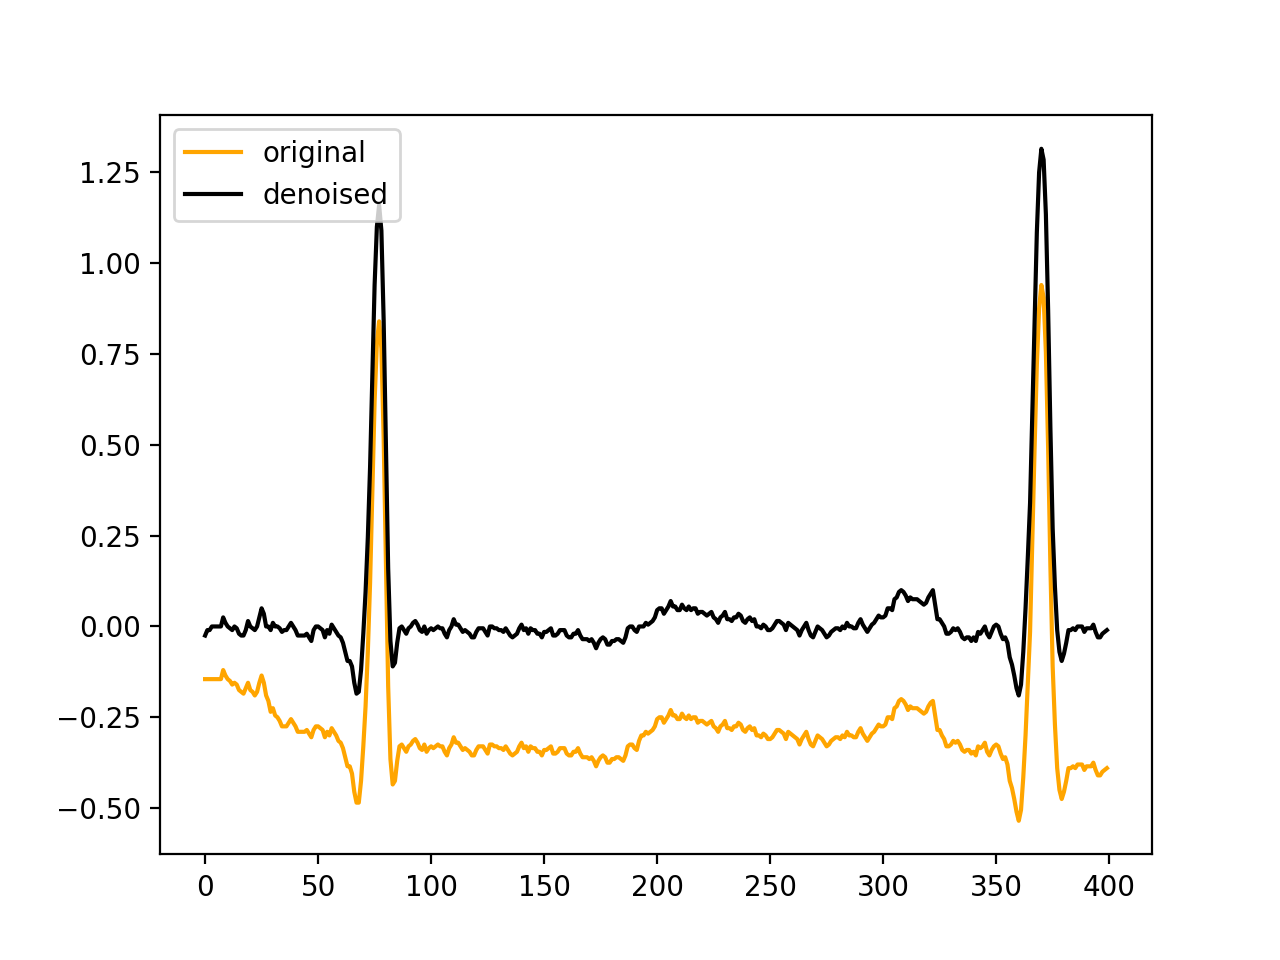
\includegraphics[width=50mm,scale=0.7]{random-forest-before-after}
	\caption{A fragment of ECG before and after the median filter}
	\label{fig:rf1}
\end{figure}
Each beat is made of a sequence of 256 samples in the RR interval, then Daubechies db2 wavelet at level 4 is applied, to obtain 265 features.\\The training set is made of 240 samples for each class and the test set of 120 for each.\\The algorithm used is Random Forest.
\begin{figure}[H]
	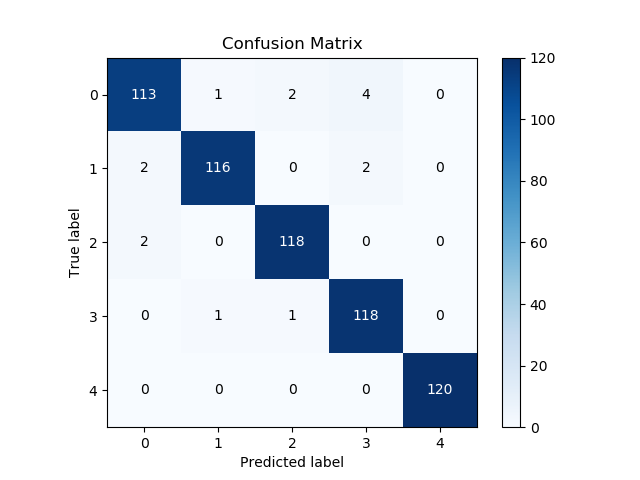
\includegraphics[width=50mm,scale=0.7]{confusion-matrix-dwt-random-forest-paper.png}
	\caption{Confusion Matrix : random forest for the N,L,R,V,P classification}
	\label{fig: rf2  }
\end{figure}
\subsection{Test}
We have executed the same approach on the original problem (N,S,V,F) classes.\\Finally, we augmented only the training dataset with SMOTE and ADASYN so that all the classes during the train had the same number of elements.
\begin{figure}[H]
	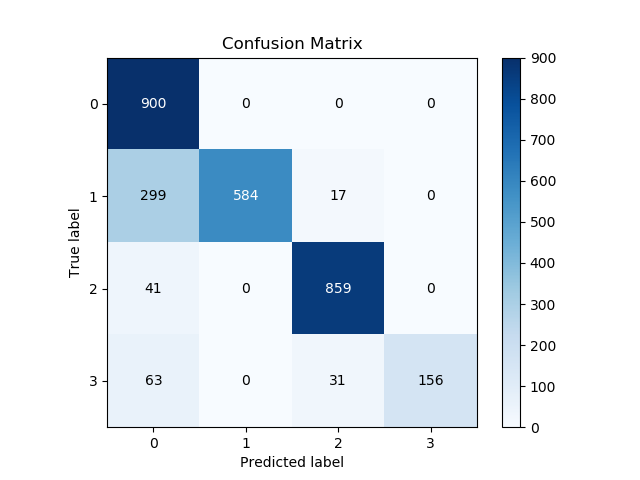
\includegraphics[width=50mm,scale=0.7]{confusion-matrixdwt-random-forest-paper-smote-smaller-test-adasyn.png}
	\caption{Confusion Matrix : random forest with adasyn for the N,S,V,F classification}
	\label{fig: rf3  }
\end{figure}
\begin{figure}[H]
	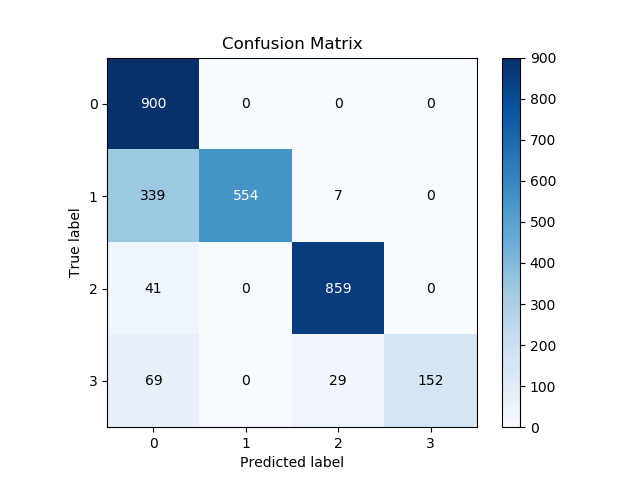
\includegraphics[width=50mm,scale=0.7]{confusion-matrixdwt-random-forest-paper-smote-smaller-test.png}
	\caption{Confusion Matrix : random forest with smote for the N,S,V,F classification}
	\label{fig: rf4  }
\end{figure}
\begin{figure}[H]
	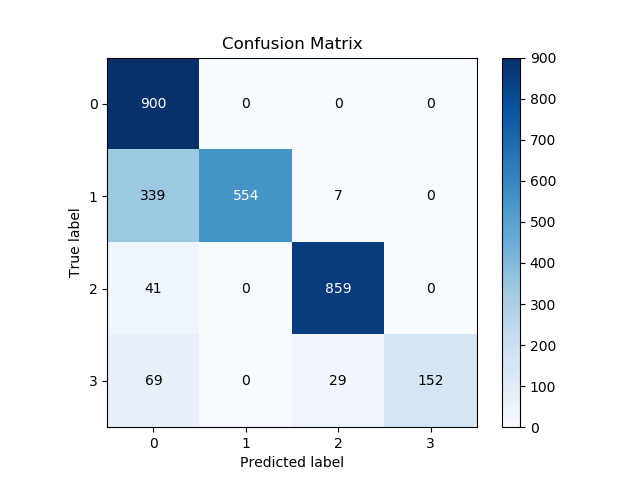
\includegraphics[width=50mm,scale=0.7]{confusion-matrixdwt-random-forest-paper-smote-smaller-no-data-aug.png}
	\caption{Confusion Matrix : random forest without data augmentation for the N,S,V,F classification}
	\label{fig: rf3  }
\end{figure}






\section{Support Vector Machine}
In this paper the de-noise is done using the discrete wavelet Daubechies db6 with nine levels and then reconstructed considering only the details coefficient from levels three to nine.Each beat is a sequence of 200 samples centered in the R peak location.
\begin{figure}[H]
	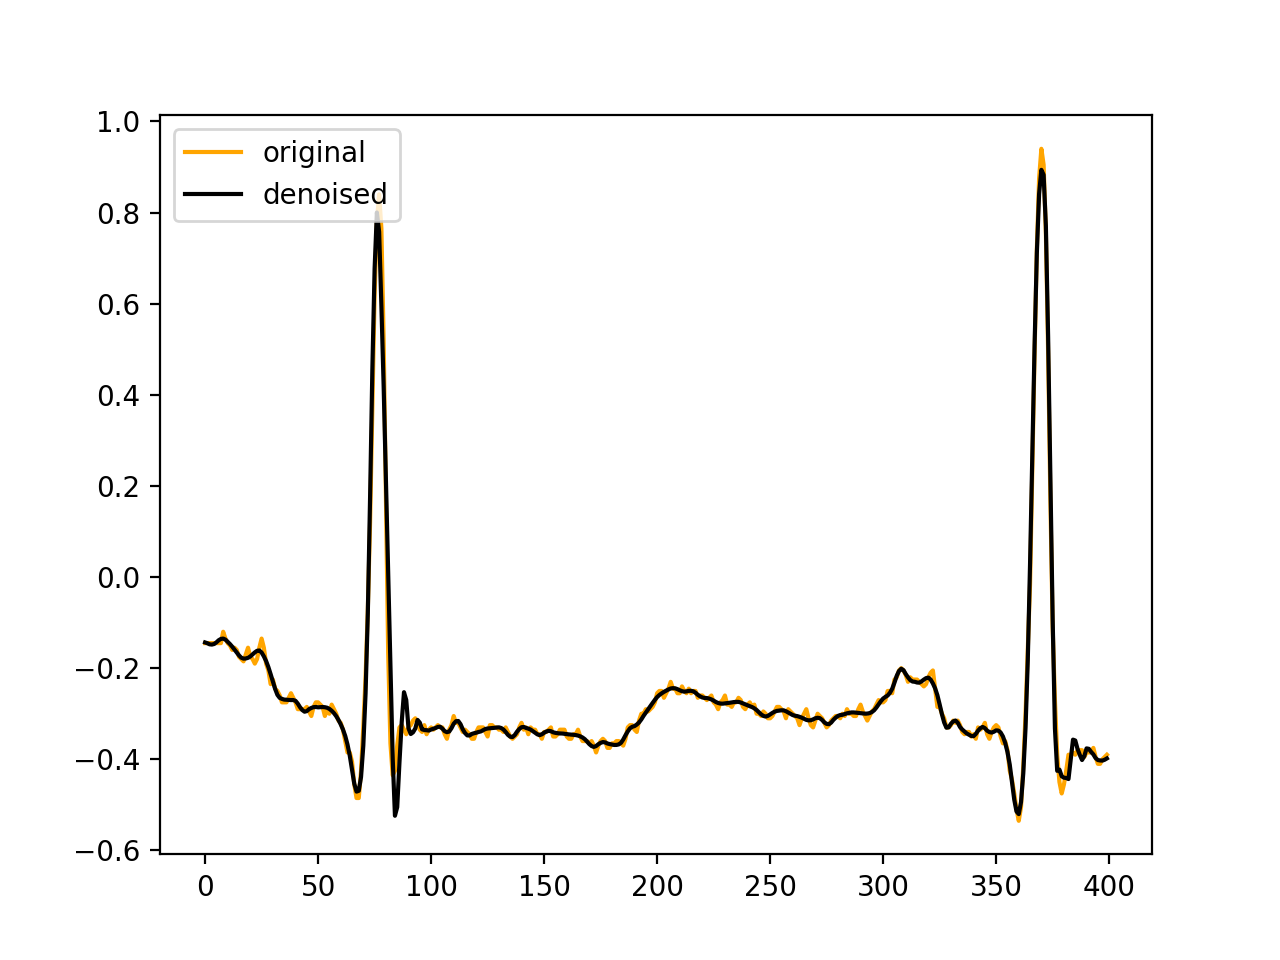
\includegraphics[width=50mm,scale=0.7]{svm-before-after}
	\caption{A fragment of ECG before and after the DWT}
	\label{fig:svc1}
\end{figure}
The features extraction consists of the following steps :
\begin{enumerate}
\item applying the discrete wavelet : Mayer with 4 levels, to each beat, to obtain in the end two matrices : one with the details coefficients of level 4 and the second one with the details coefficients of level 3 
\item applying the PCA with 6 components, respectively to the two previous matrices (12 features per beat)
\item applying the 4-th and 5-th moment to each single beat (2 features per beat)
\item applying ICA with 14 components to the matrix of beats
\end{enumerate}
The algorithm used is Support Vector Machine for classification with the following parameters:
\begin{enumerate}
% SVC(C=70,gamma=0.7,kernel='rbf',verbose=True)
\item C :  70
\item Gamma : 0.7
\item Kernel : radial basis function
\end{enumerate}
\begin{figure}[H]
	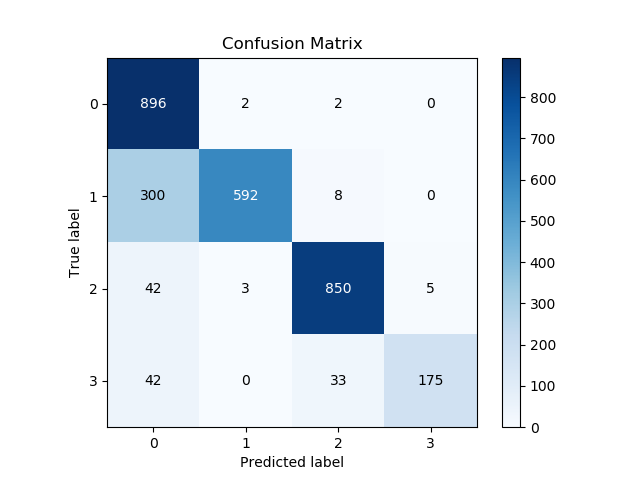
\includegraphics[width=50mm,scale=0.7]{confusion-matrix-linear-not-linear-no-aug-smaller-test.png}
	\caption{Confusion Matrix : svm for the N,S,V,F classification}
	\label{fig:svc2}
\end{figure}
\subsection{Test}
We have tested the same approach applying data augmentation with ADASYN.
\begin{figure}[H]
	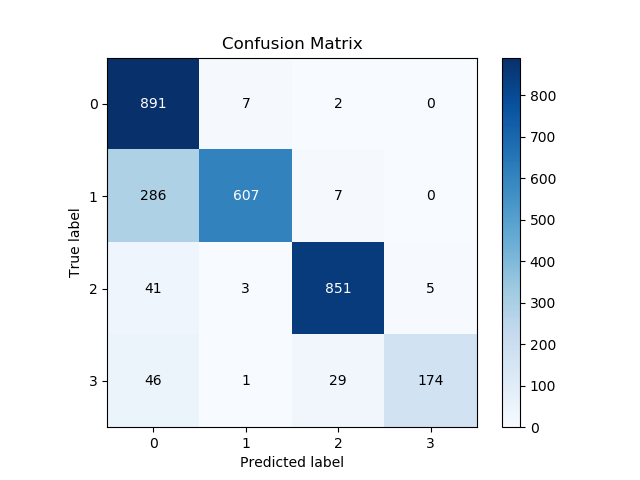
\includegraphics[width=50mm,scale=0.7]{confusion-matrix-linear-not-linear-adasyn-smaller-test.png}
	\caption{Confusion Matrix : svm with adasyn for the N,S,V,F classification}
	\label{fig:svc3}
\end{figure}
\section{CNN  \cite{5}}
This paper does not perform a real de-noising process and the pre-processing phase consists of :
\begin{enumerate}
\item resampling the signal to 125Hz (originally is 360Hz)
\item considering windows of size 10s and normalizing between 0 and 1
\item considering T as the median of the RR peak distances in time for a given signal
\item considering a beat made of a R peak and the following samples for a total size of 1.2T
\item since T is specific for a given signal, to make all beats of the same size, shorter beats are padded with zeros
\end{enumerate}
The model used is a neural network with the layers depicted in the following figure.
\begin{figure}[H]
	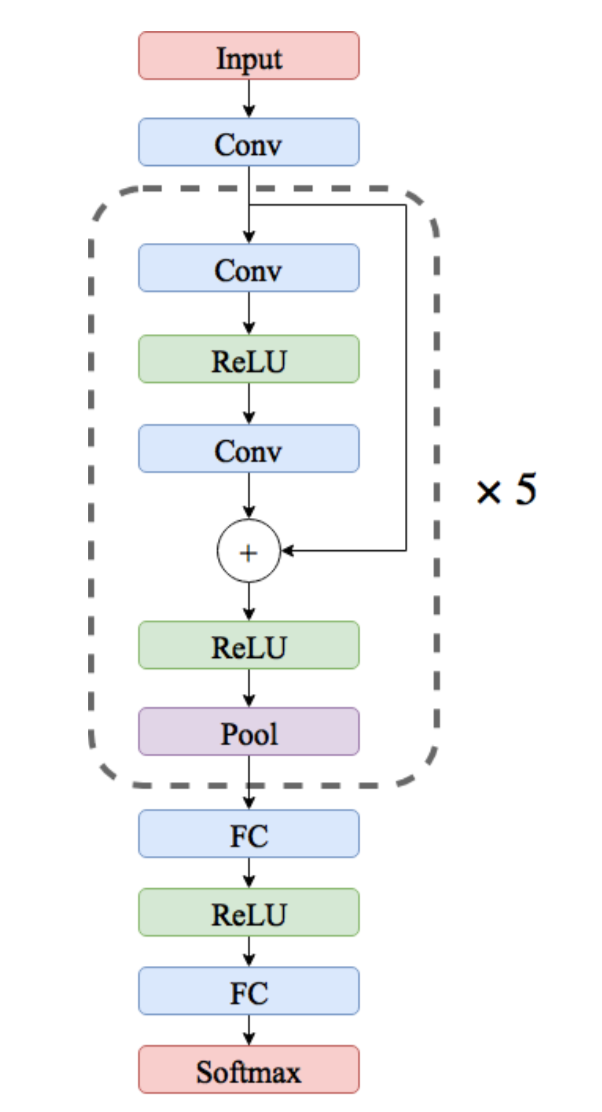
\includegraphics[width=50mm,scale=0.7]{arch-cnn}
	\caption{Architecture of the model in \cite{5}}
	\label{fig:cnn1}
\end{figure}
This approach has the benefit to have a simple pre-processing phase and it is conventional in the use of a neural network model that can be deployed in an embedded device with the support of library such as Tensorflow-Lite and uTensor.
\begin{figure}[H]
	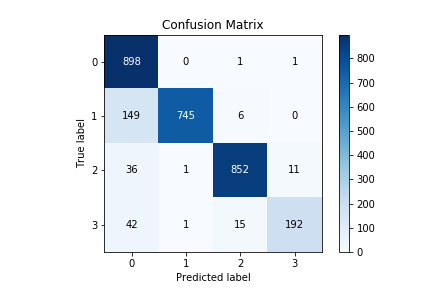
\includegraphics[width=50mm,scale=0.7]{conf-matrixno-augmentationdtrk-model.png}
	\caption{Confusion Matrix : cnn for the N,S,V,F classification}
	\label{fig:cnn1}
\end{figure}
\subsection{Test}
We have tested the same approach using ADASYN as data augmentation.\\Then we simplified the model without performing the pre-processing phase and with data augmentation.
\begin{figure}[H]
	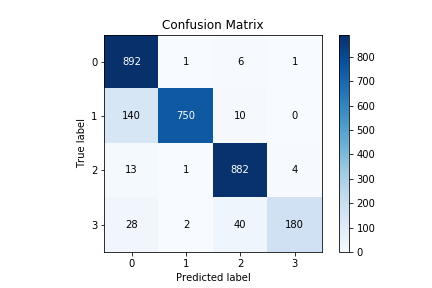
\includegraphics[width=50mm,scale=0.7]{conf-matrixADASYNdtrk-model.png}
	\caption{Confusion Matrix : cnn with adasyn for the N,S,V,F classification}
	\label{fig: cnn2}
\end{figure}
\begin{figure}[H]
	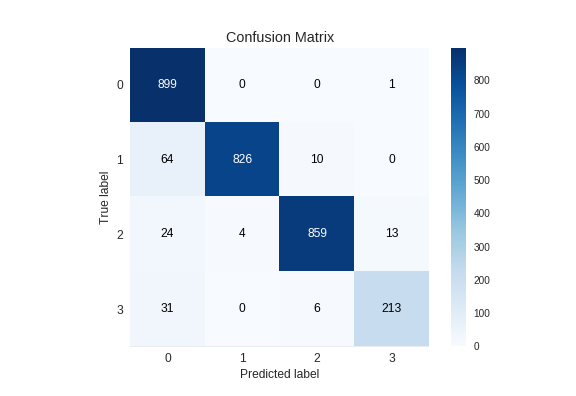
\includegraphics[width=50mm,scale=0.7]{conf-matrix-no-pre-proc-adssyn.png}
	\caption{Confusion Matrix : cnn with adasyn for the N,S,V,F classification without pre processing}
	\label{fig: cnn4}
\end{figure}







\section{Convolutional Neural Network}
\section{LSTM and Attention}
\section{Neural Ordinary Differential Equations}
\chapter{Future Work}


\backmatter
% bibliography
\cleardoublepage
\phantomsection
\bibliographystyle{sapthesis} % BibTeX style
\bibliography{biblio} % BibTeX database without .bib extension

\end{document}
